\chapter{Результаты решения задачи 3D локализации}

\section{Используемые данные}

В качестве датасета использовался не LIDC-IDRI непосредственно, как это было сделано в решении задачи 2d-сегментации, а его подможество LUNA \cite{luna}, содержащее 888 сканов в формате MetalImage и 1187 опухолей, каждая из которых представленна в виде bounding box. В отличие от LIDC-IDRI из LUNA исключены сканы, по толщине превосходящие 2.5 мм, а также включены только те опухоли, которые были размечены хотя бы тремя и четырех специалистов-радиологов. Еще одна особенность LUNA по сравнению с LIDC состоит в том, что средний размер новообразований в LUNA составляет 8.3 мм при стандартном отклонении в 4.8 мм, когда для LIDC-IDRI эти показатели составляют 12.8мм и 10.6 мм соответствено.

\section{Детали реализации}

\subsection{Реализация DeepSEED}

В оригинальной работе было предложено подавать на вход сети обрезанные участки КТ изображений размера $128^3$, однако такая размерность входных данный требует вычислительных ресурсов, которые были недоступны во время реализации, что привело к уменьшению размерности входа до $64^3$.


\subsection{Реализация Адаптивной нормализации}

Адаптивная нормализация была добавлена в сеть вместо батчевой нормализации. Она применяется после всех блоков (свертка, активация) и в кодировщике, и в декодировщике кроме первого слоя. В качестве входа $x$ формулы \eqref{eq:adain} используется тензор, полученный на выходе активации, а в качестве параметра $y$ используется выход побочной сети, имеющей простую архитектуру - 3 полносвязных слоя, причем первые два разделены между всеми побочными сетями. Данная архитектура позволяет выявить эффективные параметры афинного преобразования посредством обучения.

\subsection{Реализация CGAN}

Изначально архитектура CGAN, формат и размерность входных и выходных данных были полностью заимствованы у авторов \cite{mirsky} в качестве бейслайн решения. Отметим, что при обучении генератора авторы использовали не стандартную функцию потерь, а комбинированную:

\begin{equation}
L(o, g, D_{output}, labels) = MSE(o, g) + MAE(o, g) + L_{G}(D_{output}, labels)
\end{equation}

$o, g$ - оригинальное и генерированное изображения, соответствующие одному контексту.

$L_{GAN}$ - это стандартная функция потерь генератора, рассчитываемая на выходах дискриминатора и реальных метках объектов. Посредством уменьшения данной функции потерь генератор непосредственно стремится обмануть диксриминатор. Однако наряду с этим авторы предлагают использовать функцию потерь, минимизирующую различия между оригинальными изображениями и генерированными.

Я обучил несколько моделей с полностью заимствованными параметрами, но во время обучения и оценки результатов было обнаружено несоклько проблем:

\begin{enumerate}
    \item Функция потерь дискриминатора оптимизировалась гораздо лучше, чем функция потерь генератора, и начиная с некоторой эпохи, дискриминатор почти всегда отличал генерированные изображения от оригинальных.
    
    \item Выходные изображения были достаточно четкими в области контекста, однако в области латентного входа, где предполагалось генерировать непосредственно опухоль, изображения были мутные.
    
    \item Некоторые модели генерировали очень похожие результаты на различных входах. Данная проблема известна как mode collapse.
\end{enumerate}

Для борьбы с данными проблемами было предпринято несколько различных модификаций сети

\begin{enumerate}
    \item Вариация соотношения числа обновлений генератора и дискриминатора
    \item Увеличение размерности входа 
    \item Вариация функции потерь
\end{enumerate}

\subsubsection{Вариация соотношения числа обновлений генератора и дискриминатора}

Данный подход является стандартным для решения ситуации, когда либо генератор, либо дискриминатор отстает от другого и обучается существенно медленнее, либо совсем не обучается, и функция потерь даже возрастает. В моделях бейслайн архитектуры функции потерь и генератора и дискриминатора уменьшались, однако точность дискриминатора достигала 100\% и далее не уменьшалась. Несмотря на то, что генератору не удавалось обмануть дискриминатор, обучениие продолжало происходить в связи с присутствием $MSE$ и $MAE$ компонент. Данный подход кажется неудовлетворительным, поскольку в таком случае роль дискриминатора фактически отпадает и генератор просто стремится произвести похожее на оригинал изображение.

При увеличении соотношения числа обновлений с $1:1$ до $10:1$ в пользу генератора удалось получить визуально лучшие результаты представленные на рисунке \ref{cgan-10wu-no-adain-baseline-loss}

\begin{figure}[!h]
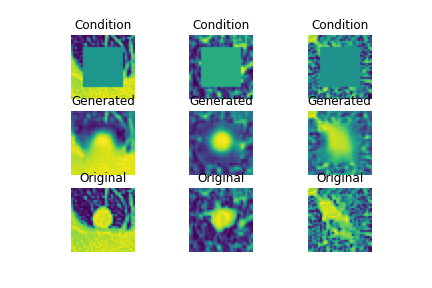
\includegraphics[width=\linewidth]{images/gan-results/no-adain.png}
\caption{Пример генерированных изображений (Без AdaIN)}\label{cgan-10wu-no-adain-baseline-loss}
\centering
\end{figure}

\subsubsection{Увеличение размерности входа}

Для избавления от проблемы mode collapse зачастую применяется увеличение латентного пространства. Если латентное пространство недостаточно велико, то модель физически не в состоянии генерировать хорошие и разнообразные изображения. Mode collapse - это состояние, когда модель отдает предпочтение одному или нескольким шаблонам и периодически меняет их, если дискриминатор подстраивается под эти шаблоны. В данном случае, так как мы используем СGAN, необходимо увеличить размерность контекста, оставляя нулевую маску в центре куба такой же.

Были предприняты попытки увеличить размерность кропов до $48^3$, то есть размерность латентного пространства увеличилась с $32^3 - 20^3$ до $48^3 - 20^3$, что кажется достаточно значительным изменением.

Однако результаты модели получились отрицательные и визуально были существенно хуже, чем для размера кропов $32^3$

\subsubsection{Wasserstein Loss}

Данный подход призван решить проблему максимальной точности, достигаемой дискриминатором. Предлагается добавить в функцию потерь Wasserstein Loss. Архитектура была настроена соответствующим образом: дискриминатор был преобразован в критика изменением выходного значения с бинарной метки на вещественное число. Тем не менее компоненту функции потерь - $MSE(original, generated)$ было решено оставить, поскольку экспериментально полученные результаты были лучше при ее наличии.

На рисунке \ref{loss} представлено изменение функции потерь в зависимости от количества обновлений генератора или критика. Заметим, что при обучении генератор обновлялся в 5 раз больше, чем критик. На рисунке видно, что генератору в целом удается обмануть критика, (в отличие от бейслайн модели), и при этом обучение сходится.

\begin{figure}[!h]
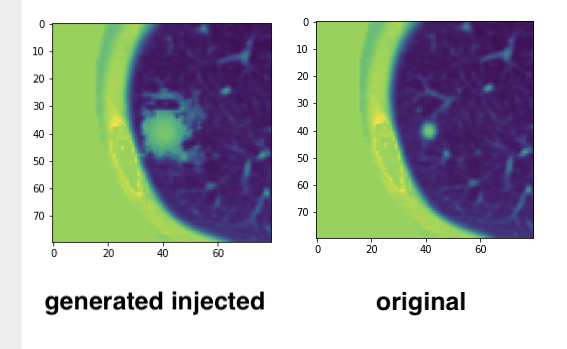
\includegraphics[width=\linewidth]{images/gan-injections/1.png}
\caption{Loss changes over time for WGAN}\label{loss}
\centering
\end{figure}

\subsubsection{Итоговая модель}
\label{section:final-gan}
В итоговую процедуру обучения вошли

\begin{enumerate}
    \item Эвристика, поддерживающая соотношение между обновлением генератора и дискриминатора, равное $5:1$ соответственно.
    \item Wasserstein Loss, комбинированный с MSE(generated, original)
    \item AdaIN (включен в модель)
\end{enumerate}

Пример генерированных итоговой моделью изображений показан на рисунке \ref{cgan-final}. На рисунке \ref{mirsky-results} представлены результаты из оригинальной работы \cite{mirsky}

\begin{figure}[!h]
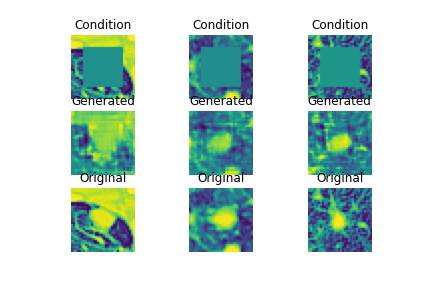
\includegraphics[width=\linewidth]{images/gan-results/final-gan.png}
\caption{Пример генерированных итоговой моделью изображений}\label{cgan-final}
\centering
\end{figure}

\begin{figure}[!h]
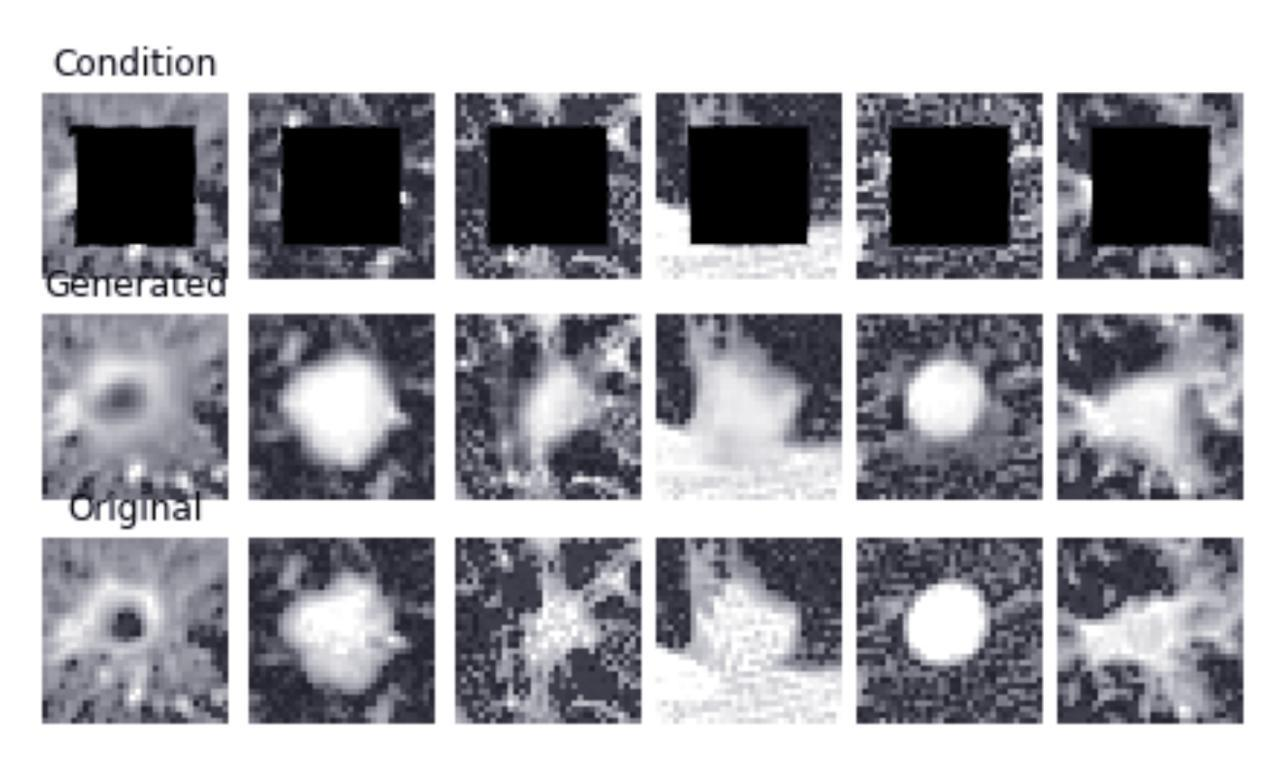
\includegraphics[width=\linewidth]{images/mirskiy-results.jpg}
\caption{Пример генерированных изображений из работы \cite{mirsky}}\label{mirsky-results}
\centering
\end{figure}

\subsection{Реализация аугментации LUNA}

Для аугментации непосредственного датасета LUNA использовалось 366 сканов из тренировочного множества, в котором всего 800 сканов, то есть процент аугментированных данных составил $31$ в итоговом экмпериментальном запуске обучения локализатора. Для аугментации использовалась модель, представленная в \ref{section:final-gan}. Участки тканей, содержащие опухоль вырезались, проходили предобработку, подавались на вход генератору, выход генератора проходил постобработку и далее вырезанные участки вставлялись обратно в скан. Процесс инъекии генерированных участков был полностью позаимствован из \cite{mirsky}.

Обратим внимание на то, каким образом выбирались участки для инъекции: было принято решение выбирать участки, содержащие настояющую опухоль. Это было сделано по нескольким причинам:

\begin{enumerate}
    \item Таким образом не нарушаются пространственные признаки участков опухоли в используемых данных (то есть мы не будем вставлять опухоль туда, где она биологически маловероятно может появиться)
    \item Поскольку мы использовали WGAN, а не оригинальную модель, генерируемые опухоли в гораздо меньшей степени напоминают оригинальные при таком же контексте, то есть разнообразие и случайность опухолей достаточно велики
    \item Обнаружение мест, пригодных для инъекции, не является простой задачей и требует либо решения дополнительной задачи сегментации и валидации ее результатов, либо ручной разметки.

\end{enumerate}


На рисунке \ref{injection} показан пример генерированной опухоли, вставленной в скан, по сравнению с оригинальной. Стоит упомянуть, что так как обучение GAN происходило на отобранных опухолях диаметра не меньше 10мм и не больше 16мм, размер генерированной опухоли несколько больше, чем оригинальной.

\begin{figure}[!h]
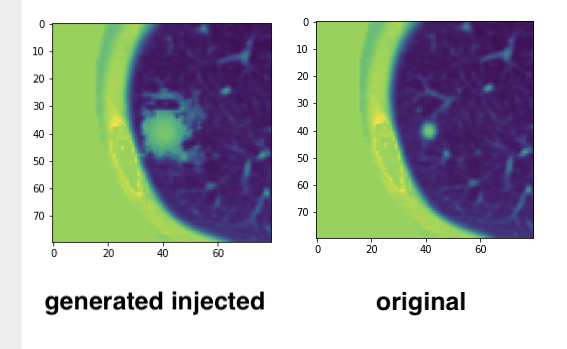
\includegraphics[width=\linewidth]{images/gan-injections/1.png}
\caption{Пример опухоли, вставленной в скан}\label{injection}
\centering
\end{figure}

\section{Результаты}

\subsection{Результаты локализации}

Оценка качества моделей производится с помощью несколько измененного FROC анализа, представленного в официальном скрипте LUNA Challenge \cite{luna} и широко используемого в работах по локализации новообразований в легких (в частности в работе \cite{li2019deepseed}). Оценка модели представлена набором точек, формирующих FROC кривую, где каждая точка представляет среднее количество ложно положительных предсказаний на один скан (average fp / scan) - по оси x - и соответствующую ему чувствительность - по оси y. Отметим, что классический FROC-анализ не был произведен, поскольку в методе оценки (average fp  / scan) \cite{luna} модели предполагается подавать на вход кропы большого  размера, а именно $208^3$, что невозможно в рамках текущей работы по причине недостатка вычислительных мощностей.

В связи с этой проблемой было решено произвести аналогичный анализ, но по оси x будут отмечены средние значения количества ложно положительных предсказаний на один кроп размера $64^3$. Уместность данного анализа обоснована тем, что каждая точка на оси x соответствует некоторому значению порога модели, контролирующего среднее число ложно-положительных предсказаний, которые склонна находить модель. Так как основной задачей работы является аугментация данных с помощью GAN, интересно в первую очередь оценить относительный выигрыш в локализации при использовании аугментированных данных в обучении.

Приведем метрики для полученных моделей в виде таблицы \ref{tab:result-metrics} и графика \ref{image:final-results}


\begin{table}[!h]
\caption{Численные результаты}\label{tab:result-metrics}
\centering
\begin{tabular}{|*{18}{c|}}\hline
\textbf{Модель} & \textbf{0.25} & \textbf{0.5} & \textbf{1} & \textbf{2} & \textbf{4} & \textbf{8} \\\hline
Без аугментации, 100 эпох & 0.44 & 0.56 & 0.65 & 0.78 & 0.85 & 0.87 \\\hline
С аугментацией, 100 эпох & 0.48 & 0.58 & 0.71 & 0.81 & 0.88 & 0.9 \\\hline
\end{tabular}
\end{table}

\begin{figure}[!h]
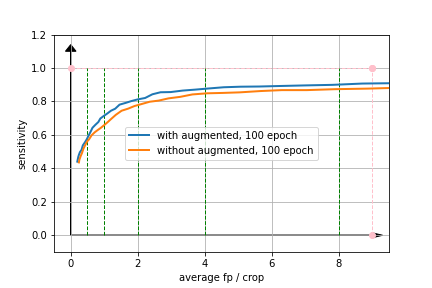
\includegraphics[width=\linewidth]{images/result_plot.png}
\caption{Итоговые FROC (over crop) кривые}\label{image:final-results}
\centering
\end{figure}


\begin{figure}[!h]
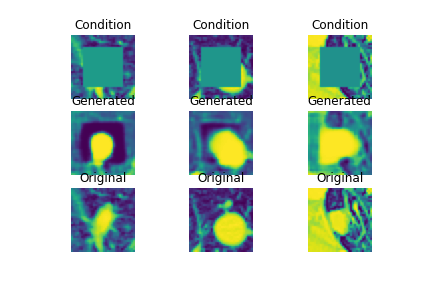
\includegraphics[width=\linewidth]{images/gan-results/adain.png}
\caption{Пример генерированных изображений (С использованием AdaIN)}\label{cgan-adain-results}
\centering
\end{figure}

\subsection{Сравнение результатов с другими работами}

Проведем сравнение с работой \cite{han2019synthesizing}, в которой были произведена аналогичная аугментация, однако использовался LIDC-IDRI вместо LUNA, в качестве модели локализации использовалась Faster-RCNN, а в качестве GAN - MCGAN c 4-мя сверточными слоями в кодировщике и 4-мя в декодировщике, а также skip-связями. Дискриминатор по своей структуре похож на Pix2Pix GAN, а в качестве функции потерь использовался Wasserstein Loss (с Gradient Penalty) наряду с Least Squares Loss. На вход подавались данные размера $64^3$, где середина размера $32^3$ заменялась случайным шумом, что существенно увеличивает размерность латентного пространства по сравнению с нашей моделью.

На рисунке \ref{han-froc-plot} приведены графики, а на рисунке \ref{han-cpm} численные результаты. CPM (Competition Performance Metric) представляет из себя усредненную чувствительность по (0.125, 0.25, 0.5, 1, 2, 4, 8) значениям average fp / scan.

\begin{figure}[!h]
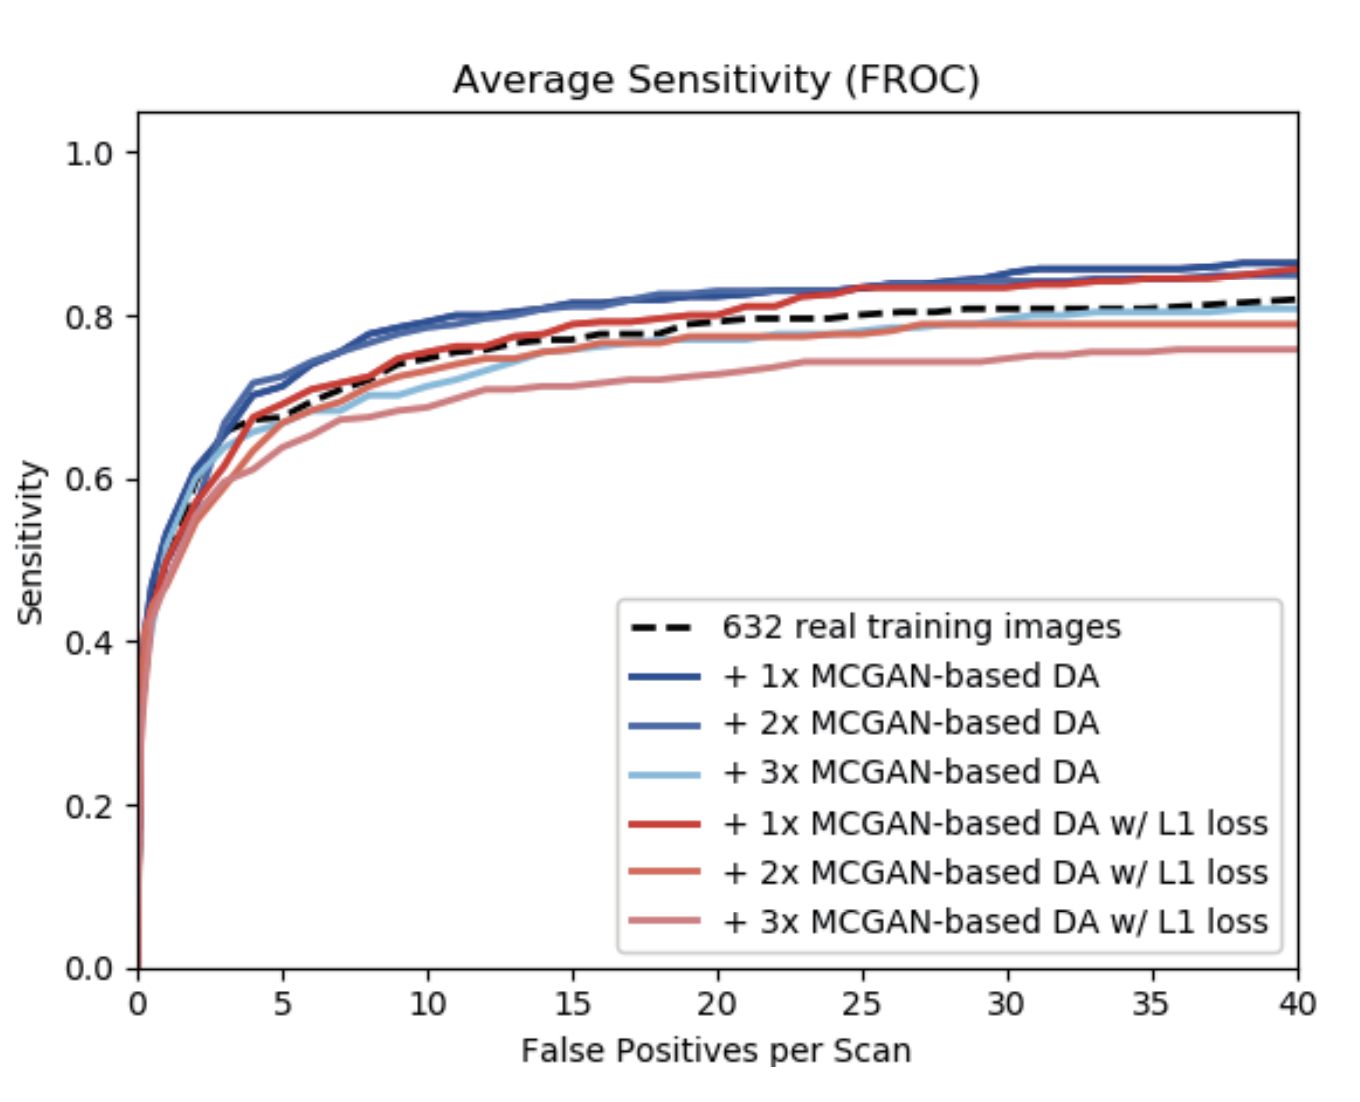
\includegraphics[width=\linewidth]{images/mcgan-results.png}
\caption{График FROC-кривой из работы \cite{han2019synthesizing}}\label{han-froc-plot}
\centering
\end{figure}

\begin{figure}[!h]
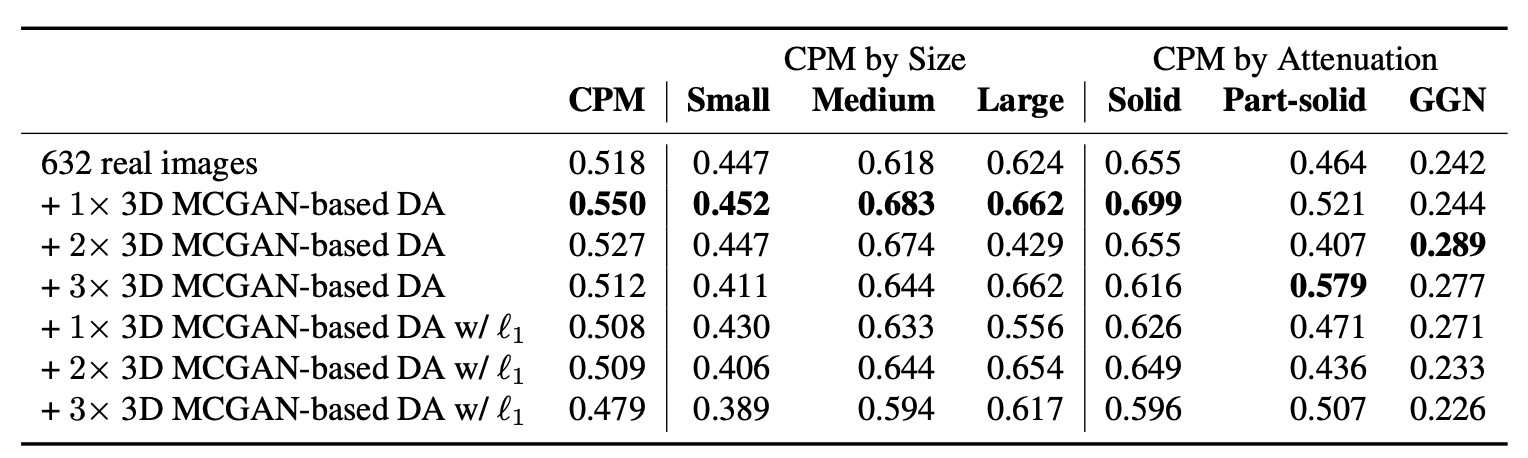
\includegraphics[width=\linewidth]{images/han-cpm.png}
\caption{Численные результаты работы \cite{han2019synthesizing}}\label{han-cpm}
\centering
\end{figure}